\begin{figure*}
  \centering
  \resizebox{1.5\columnwidth}{!}{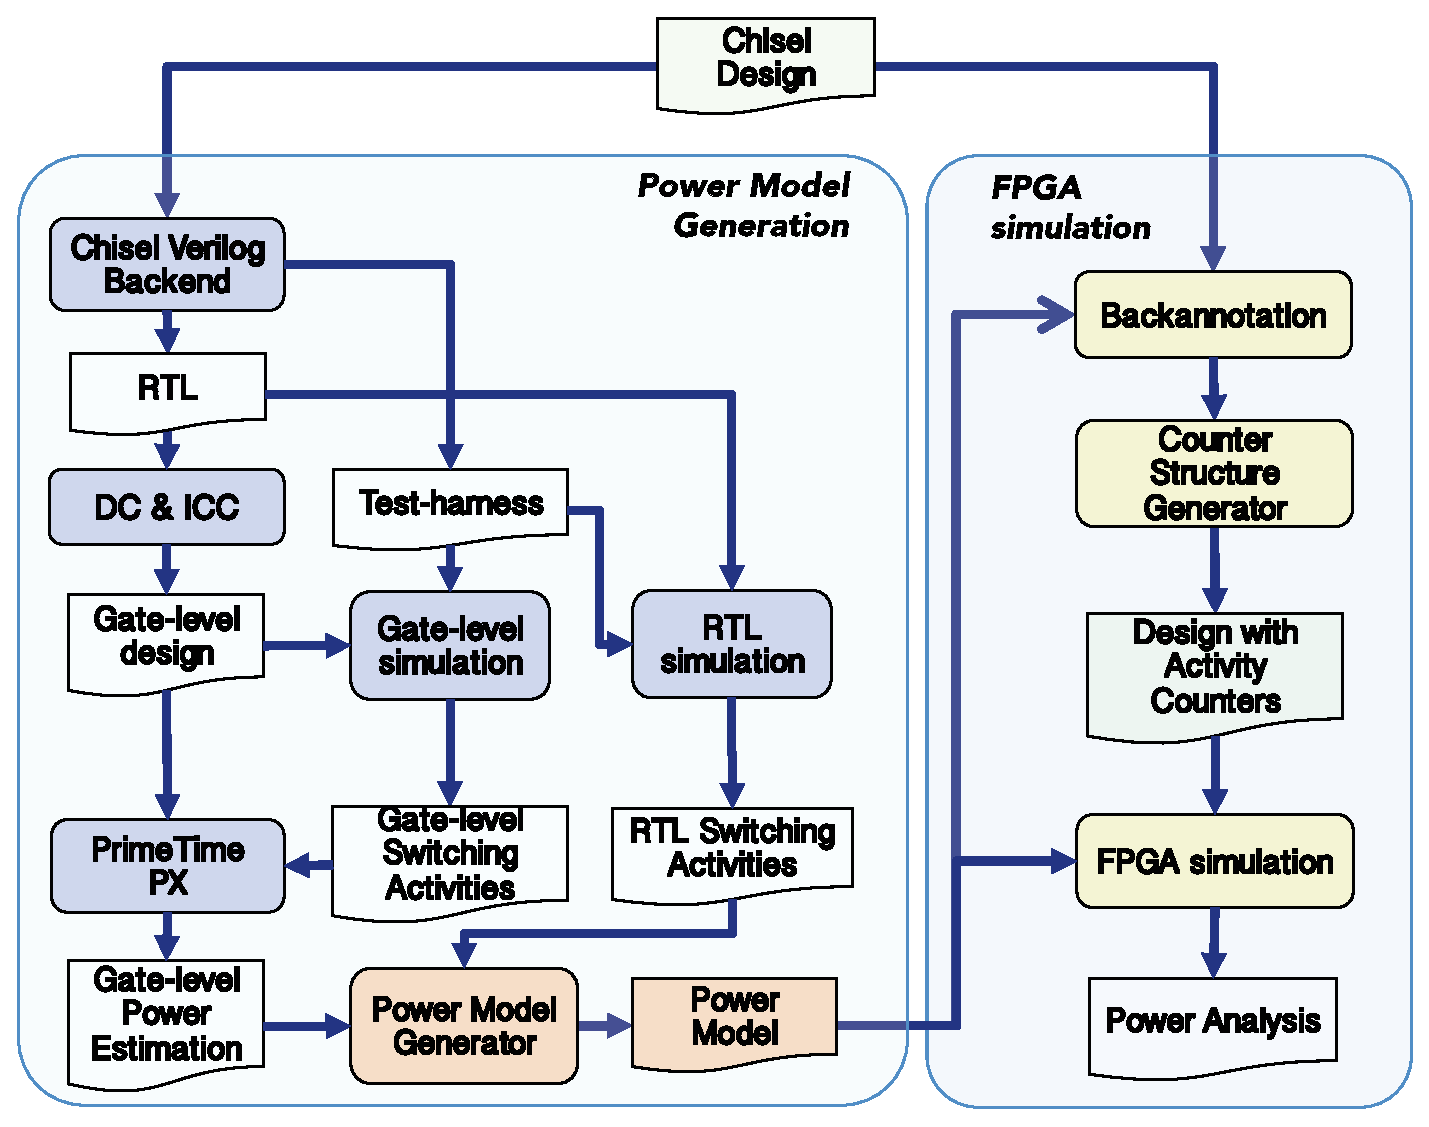
\includegraphics{figure/toolflow}}
  \caption{Tool flow for FPGA-accelerated power simulation}
  \label{fig:toolflow}
\end{figure*}

\section {Tool Flow}
Fig. \ref{fig:toolflow} shows the entire flow for FPGA-accelerated power simulation consisting of two major paths.
We assume that both paths start from the Chisel design.

The left-hand side path is to automatically generate the power models for the target design.
Basically, the power model generator not only approximates the gate-level power estimation with the RTL switching activities,
but also selects the significant RTL signals in the power analysis.

The chisel design is compiled to the RTL design by the Chisel verilog backend,
and to the the gate-level design by the design compiler and the IC compiler.
PrimeTime PX estimates the gate-level power consumption using the gate-level design and its switching activities from gate-level simulation.
In addition, RTL simulation provides the RTL switching activities.
The gate-level power numbers and the RTL switching activities are the inputs for the power model generator.

The power model generator provides the design's linear power model.
It finds the linear relationship between the RTL switching activities and the power consumption of the target design.
To make power measuring tractable, the power generator has to pick the dominant signals in the power model.
The way the power model generator works is explained in Section \ref{sec:main} in detail.

The right-hand side path is to automatically generate the counter structure for FPGA simulation.
FPGA simulation should provide the selected signal activities to calculate the design's power consumption using the power model.
Thus, the Chisel backend backannotates the selected signals from the power model, and generates the activity counter structure.
The design with the activity counters is ported to FPGA, and then FPGA simulation provides the signals' activities from the counter structure.
This enables the detailed power analysis for the target design with its various applications.